\setcounter{secnumdepth}{4}
\subsection{Abnormality Detection and Localization in Chest X-Rays using Deep Convolutional Neural Networks}

For this paper, researchers conducted experiments on three datasets. From the datasets, researchers explored the performance of various deep CNN's for detection of heart disease from chest X-rays. Researchers used binary classification on diseases such as Cardiomegaly against normal images \cite{islam2017abnormality}. The paper explores several CNN models such as AlexNet, VGG-Net and ResNet. These models have different layers and typically achieve higher accuracy as layers increase as noted in State-of-the-Art section.

Another part of the research, similar to previous papers reviewed was to produce a heat-map showing which areas of the X-ray the model has the highest activation on. This paper used the sensitivity of softmax scores of occlusion on a certain region in the chest X-ray to find which region in the image is responsible for the classification decision.  
\subsubsection {Results}

The first experiment used single model CNN's on the Indiana dataset, and from the tests, it was shown that deeper models like VGG-19, ResNet improve the accuracy significantly. It was found that Cardiomegaly detection improves 6\% compared to using shallower models like AlexNet. Although results showed high specificity for ResNet-101 and high sensitivity for VGG-16, the VGG-19 gave the highest AUC score of 0.94. This at least 1\% higher AUC for other models. 
As well as this, dropout was used, which increased performance on the shallower networks but degraded deeper ones. For all experiments, it was noted that extracting features from earlier layers lead to improved accuracy of 2-4\%. It was concluded that shallower networks were better for detecting smaller objects, and as an example, it was found that shallower layers from ResNet-15 trained on Cardiomegaly had better performance than later layers across different metrics. figure~\ref{fig:Shallow} shows a more in depth picture of findings. 

\begin{figure}[H]
	\centering
	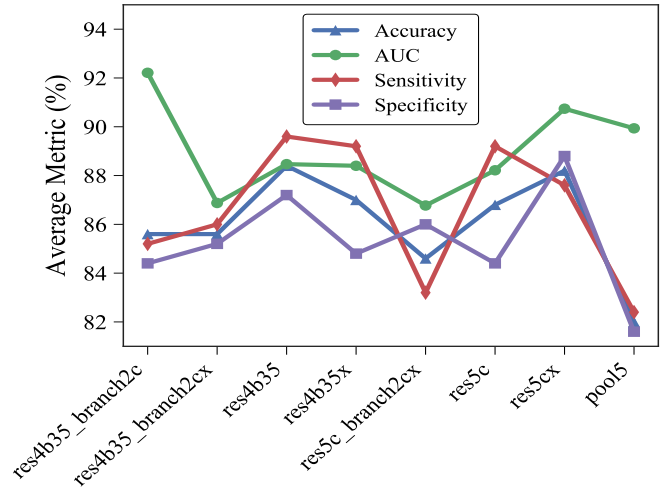
\includegraphics[scale=0.7]{ShallowerLayers.png}
	\caption{Researchers showed that shallower layers in models had a higher accuracy on Cardiomegaly detection compared to deep layers}
	\label{fig:Shallow}
\end{figure}

Another fascinating result was on the localisation of Cardiomegaly shown in the image below. It can be observed that from the figure~\ref{fig:Cardiomegaly}, the model has higher activations from the heart region, which is expected as Cardiomegaly concerns abnormal enlargement of the heart. What was revealing was that other than an enlarged heart for a patient with Cardiomegaly, there is not much difference in features between a normal image and an image classified as Cardiomegaly. But the model can still differentiate between a normal heart which is enlarged due to age or physical attributes of the patient. 
\begin{figure}[H]
	\centering
		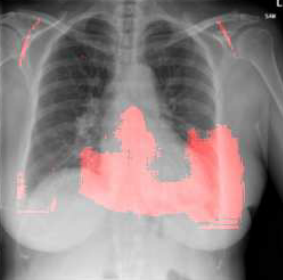
\includegraphics[scale=0.7]{CardiomegalyMap.png}
	\caption{Occlusion sensitivity used to create heap map of region where it thinks Cardiomegaly exists }
	\label{fig:HeatMap}
\end{figure}

\begin{figure}[H]
	\centering
	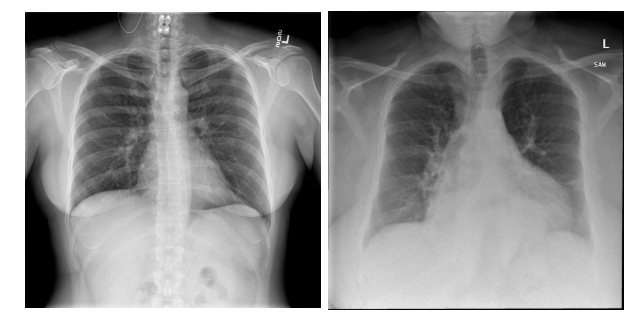
\includegraphics[scale=0.7]{NormalVsCardiomegaly.png}
	\caption{Example of normal heart on the left and Cardiomegaly diagnosed heart on the right }
	\label{fig:Cardiomegaly}
\end{figure}



Finally, another point raised in the paper was the model used for localisation of cardiomegaly were counter-intuitive to traditional methods of cardiomegaly diagnosis, which consider the relative size of heart and lung. But, most of the signals contributing to the softmax score come from the heart alone indicating features in the shape of the heart and its surrounding region alone help in detection of the pathology and perhaps the lung and relative size to the heart are less critical in the diagnosis for the model. 
 

 
 



